\paragraph{Mô hình động học phân tử về cấu tạo chất và chuyển động Brown}
%%----------Câu mới----------%%

\dangbt{Mô hình động học phân tử về cấu tạo chất và chuyển động Brown}
\begin{ex}
% Mức: NB
% ID: L12C1B1-82-TN
	{\color{red}\footnotesize\ttfamily [L12C1B1-TN-42]}\par %HienID
	Chuyển động Brown là
	\choice
	{chuyển động có quỹ đạo xác định của các phân tử chất lỏng}
	{\True chuyển động hỗn loạn, không ngừng của các hạt nhỏ (như hạt phấn hoa) lơ lửng trong chất lỏng hoặc chất khí, do bị các phân tử môi trường va chạm}
	{sự rung động tại chỗ của nguyên tử trong mạng tinh thể chất rắn}
	{sự khuếch tán có quy luật của các phân tử khí trong chất lỏng}
	\loigiai{
		Chuyển động Brown là chuyển động hỗn loạn, không ngừng của các hạt rất nhỏ lơ lửng trong chất lỏng hoặc chất khí, gây ra bởi sự va chạm không cân bằng liên tục của các phân tử môi trường xung quanh vào hạt đó.
		Kết luận: Phương án đúng là ý (2).
	}
\end{ex}
%%----------Câu mới----------%%
\begin{ex}
% Mức: TH
% ID: L12C1B1-83-TN
	{\color{red}\footnotesize\ttfamily [L12C1B1-TN-43]}\par %HienID
	Chuyển động Brown là bằng chứng thực nghiệm chứng tỏ điều gì về các phân tử chất lỏng, chất khí?
	\choice
	{Các phân tử đứng yên tại các vị trí cố định}
	{\True Các phân tử chuyển động hỗn loạn, không ngừng}
	{Các phân tử chỉ chuyển động khi có ánh sáng chiếu vào}
	{Các phân tử sắp xếp có trật tự chặt chẽ}
	\loigiai{
		Thí nghiệm của Brown quan sát thấy hạt phấn hoa lơ lửng trong nước chuyển động hỗn loạn không ngừng dù không chịu tác động bên ngoài nào khác, điều này chứng tỏ các phân tử nước xung quanh hạt phấn hoa luôn chuyển động hỗn loạn, không ngừng và va chạm vào hạt phấn hoa từ mọi phía.
		Kết luận: Các phân tử chuyển động hỗn loạn, không ngừng.
	}
\end{ex}
%%----------Câu mới----------%%
\begin{ex}
% Mức: NB
% ID: L12C1B1-84-TN
	{\color{red}\footnotesize\ttfamily [L12C1B1-TN-44]}\par %HienID
	Khi nhiệt độ của một khối chất tăng lên, tốc độ chuyển động hỗn loạn trung bình của các phân tử cấu tạo nên chất đó sẽ
	\choice
	{giảm xuống}
	{không đổi}
	{\True tăng lên}
	{bằng không}
	\loigiai{
		Theo mô hình động học phân tử, nhiệt độ của vật càng cao thì tốc độ chuyển động (chuyển động nhiệt) của các phân tử cấu tạo nên vật càng lớn.
		Kết luận: Tốc độ chuyển động hỗn loạn trung bình của các phân tử tăng lên.
	}
\end{ex}
%%----------Câu mới----------%%
\begin{ex}
% Mức: NB
% ID: L12C1B1-85-TN
	{\color{red}\footnotesize\ttfamily [L12C1B1-TN-45]}\par %HienID
	Trong thí nghiệm của Brown (năm 1827), đối tượng được quan sát trực tiếp dưới kính hiển vi là
	\choice
	{các phân tử nước}
	{\True các hạt phấn hoa rất nhỏ lơ lửng trong nước}
	{các ion hòa tan trong nước}
	{các phân tử khí hòa tan trong nước}
	\loigiai{
		Brown đã quan sát các hạt phấn hoa rất nhỏ lơ lửng trong nước bằng kính hiển vi và thấy chúng chuyển động hỗn loạn, không ngừng — hiện tượng này về sau được gọi là chuyển động Brown. Bản thân các phân tử nước có kích thước quá nhỏ để có thể quan sát trực tiếp bằng kính hiển vi quang học thời đó.
		Kết luận: Đối tượng quan sát trực tiếp là các hạt phấn hoa rất nhỏ lơ lửng trong nước.
	}
\end{ex}



%%----------Câu 8----------%%
\begin{ex}
% Mức: TH
% ID: L12C1B1-86-TN
	{\color{red}\footnotesize\ttfamily [L12C1B1-TN-2]}\par %HienID
	Phát biểu nào \textbf{không} đúng với mô hình động học phân tử?
	\choice
	{Giữa các phân tử có lực tương tác gọi là lực liên kết phân tử}
	{\True Tốc độ chuyển động của các phân tử cấu tạo nên vật càng lớn thì thể tích của vật càng lớn}
	{Các chất được cấu tạo từ các hạt riêng biệt là phân tử}
	{Các phân tử chuyển động không ngừng}
	\loigiai{
		\begin{itemize}
			\item Tốc độ chuyển động của các phân tử cấu tạo nên vật càng lớn thì nhiệt độ càng lớn.
	\end{itemize}}
\end{ex}

%%----------Câu 9----------%%
\begin{ex}
% Mức: NB
% ID: L12C1B1-87-TN
	{\color{red}\footnotesize\ttfamily [L12C1B1-TN-17]}\par %HienID
	Theo mô hình động học phân tử về cấu tạo chất thì các chất được cấu tạo từ các hạt riêng biệt là
	\choice
	{ion}
	{plasma}
	{nguyên tử}
	{\True phân tử}
	\loigiai{Vật chất được cấu tạo từ bởi 1 số rất lớn những hạt có kích thước rất nhỏ gọi là phân tử}
\end{ex}

\paragraph{Phân biệt đặc điểm cấu trúc phân tử của chất ở thể rắn, lỏng, khí}

%%----------Câu 10----------%%
\begin{ex}
% Mức: TH
% ID: L12C1B1-88-TN
	{\color{red}\footnotesize\ttfamily [L12C1B1-TN-4]}\par %HienID
	Chất rắn có hình dạng nhất định vì các phân tử trong chất rắn
	\choice
	{\True được liên kết chặt chẽ và có trật tự}
	{có thể di chuyển tự do}
	{bị hút về phía trung tâm bởi lực hấp dẫn mạnh}
	{được sắp xếp ngẫu nhiên và rời rạc}
	\loigiai{Các phân tử trong thể rắn có thứ tự sắp xếp trật tự chặc chẽ, lực tương tác mạnh, không cho di chuyển tự do, chỉ có thể dao động quanh vị trí cân bằng xác định}
\end{ex}

%%----------Câu 11----------%%
\begin{ex}
% Mức: TH
% ID: L12C1B1-89-TN
	{\color{red}\footnotesize\ttfamily [L12C1B1-TN-6]}\par %HienID
	Đặc điểm nào sau đây là đúng với cấu trúc của chất ở thể lỏng?
	\choice
	{Các phân tử có lực tương tác rất yếu}
	{Các phân tử chuyển động hỗn loạn và có khoảng cách rất lớn}
	{Giữa các phân tử không có khoảng cách}
	{\True Các phân tử dao động quanh vị trí cân bằng, vị trí cân bằng có thể dịch chuyển}
	\loigiai{Các chất ở thể lỏng có các phân tử dao động quanh vị trí cân bằng, vị trí cân bằng có thể dịch chuyển.}
\end{ex}

%%----------Câu 12----------%%
\begin{ex}
% Mức: TH
% ID: L12C1B1-90-TN
	{\color{red}\footnotesize\ttfamily [L12C1B1-TN-9]}\par %HienID
	Hình vẽ dưới đây mô tả, so sánh khoảng cách và sự sắp xếp các phân tử ở các thể khác nhau (a), chuyển động của phân tử ở các thể khác nhau (b). Hình nào mô tả cấu trúc của thể rắn?
	\begin{center}
		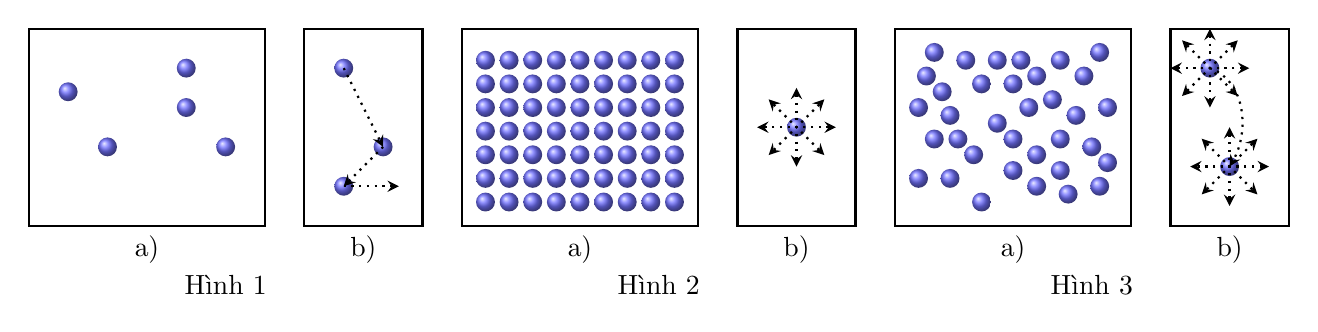
\begin{tikzpicture}[>=stealth, thick]
			
			\draw (0,0) rectangle (3,2.5)
			(3.5,0) rectangle (5,2.5);
			
			\foreach \x/\y in {1/1, 0.5/1.7, 2/2, 2/1.5, 2.5/1} {
				\shade[ball color=blue!60, opacity=0.95] (\x,\y) circle (0.12cm);
			}
			
			\foreach \x/\y in {4/2, 4.5/1, 4/0.5} {
				\shade[ball color=blue!60, opacity=0.95] (\x,\y) circle (0.12cm);
			}
			
			\node[below] at (1.5,0) {a)};
			\node[below] at (4.25,0) {b)};
			\node[below] at (2.5,-0.5) {Hình 1};
			
			\draw[->, dotted] (4,2) -- (4.5,1);
			\draw[->, dotted] (4.5,1) -- (4,0.5);
			\draw[->, dotted] (4,0.5) -- (4.7,0.5);
			
			\begin{scope}[shift={(5.5,0)}]
				\draw (0,0) rectangle (3,2.5)
				(3.5,0) rectangle (5,2.5);
				
				\node[below] at (1.5,0) {a)};
				\node[below] at (4.25,0) {b)};
				\node[below] at (2.5,-0.5) {Hình 2};
				
				\foreach \x in {0.3,0.6,...,3.0}{
					\foreach \y in {0.3,0.6,...,2.4}{
						\shade[ball color=blue!60, opacity=0.95] (\x,\y) circle(0.12cm);
					}
				}
				
				\shade[ball color=blue!60, opacity=0.95] (4.25,1.25) circle(0.12cm);
				
				\foreach \x/\y in {0/180,45/-135,90/-90,135/-45}{
					\draw[<->, dotted]
					({4.25+0.5*cos(\x)},{1.25+0.5*sin(\x)})
					-- ({4.25+0.5*cos(\y)},{1.25+0.5*sin(\y)});
				}
			\end{scope}
			
			\begin{scope}[shift={(11,0)}]
				\draw (0,0) rectangle (3,2.5)
				(3.5,0) rectangle (5,2.5);
				
				\node[below] at (1.5,0) {a)};
				\node[below] at (4.25,0) {b)};
				\node[below] at (2.5,-0.5) {Hình 3};
				
				\foreach \x/\y in {
					0.7/0.6, 1.5/1.1, 1.8/1.9, 1.5/0.7, 2.5/1.0,
					1.1/1.8, 0.8/1.1, 1.1/0.3, 2.1/1.1, 0.5/1.1,
					0.7/1.4, 2.6/0.5, 2.7/1.5, 1.3/1.3, 0.9/2.1,
					1.5/1.8, 1.8/0.5, 2.4/1.9, 0.3/0.6, 0.4/1.9,
					1.0/0.9, 2.0/1.6, 1.3/2.1, 1.7/1.5, 2.6/2.2,
					2.1/2.1, 2.2/0.4, 2.1/0.7, 1.8/0.9, 2.3/1.4,
					0.3/1.5, 0.6/1.7, 1.6/2.1, 2.7/0.8, 0.5/2.2
				}{
					\shade[ball color=blue!60, opacity=0.95] (\x,\y) circle(0.12cm);
				}
				
				\shade[ball color=blue!60, opacity=0.95] (4,2) circle(0.12cm);
				\shade[ball color=blue!60, opacity=0.95] (4.25,0.75) circle(0.12cm);
				
				\foreach \x/\y in {0/180,45/-135,90/-90,135/-45}{
					\draw[<->, dotted] 
					({4+0.5*cos(\x)},{2+0.5*sin(\x)}) -- ({4+0.5*cos(\y)},{2+0.5*sin(\y)});
					\draw[<->, dotted] 
					({4.25+0.5*cos(\x)},{0.75+0.5*sin(\x)}) -- ({4.25+0.5*cos(\y)},{0.75+0.5*sin(\y)});
				}
				
				\draw[->, dotted] (4,2) [out=-20,in=60] to (4.25,0.75);
				
			\end{scope}
			
		\end{tikzpicture}
		
	\end{center}
	\choice
	{\True Hình $(2)$}
	{Hình $(1)$}
	{Hình $(3)$}
	{Hình $(2)$ và $(3)$}
	\loigiai{Các phân tử trong thể rắn có thứ tự sắp xếp trật tự chặc chẽ, lực tương tác mạnh, không cho di chuyển tự do, chỉ có thể dao động quanh vị trí cân bằng xác định}
\end{ex}


%%----------Câu mới----------%%
\begin{ex}%[L12C1B1-DS-13]
	{\color{red}\footnotesize\ttfamily [L12C1B1-DS-13]}\par %HienID
	Xét các phát biểu về mô hình động học phân tử và chuyển động Brown.
	\choiceTF[t]
	{Mô hình động học phân tử cho rằng vật chất được cấu tạo liên tục, không có khoảng trống giữa các hạt}
	{\True Chuyển động Brown là bằng chứng thực nghiệm cho thấy các phân tử chất lỏng (hoặc khí) chuyển động hỗn loạn không ngừng}
	{\True Nhiệt độ của môi trường càng cao thì chuyển động Brown của hạt quan sát được càng mạnh (nhanh) hơn}
	{Chuyển động Brown chỉ xảy ra đối với các hạt có kích thước bằng đúng kích thước của một phân tử}
	\loigiai{
		\begin{itemchoice}
			\item Mô hình động học phân tử cho rằng vật chất được cấu tạo từ các hạt riêng biệt (gián đoạn), giữa các hạt luôn có khoảng cách chứ không phải cấu tạo liên tục. Mệnh đề sai.
			\item Hiện tượng hạt phấn hoa chuyển động hỗn loạn, không ngừng trong thí nghiệm của Brown chỉ có thể giải thích được nếu thừa nhận các phân tử chất lỏng xung quanh cũng đang chuyển động hỗn loạn, không ngừng và va chạm vào hạt phấn hoa. Mệnh đề đúng.
			\item Khi nhiệt độ môi trường tăng, tốc độ chuyển động nhiệt của các phân tử chất lỏng tăng lên, làm tần suất và cường độ va chạm vào hạt quan sát tăng, khiến chuyển động Brown của hạt diễn ra càng mạnh (nhanh) hơn. Mệnh đề đúng.
			\item Chuyển động Brown thường được quan sát ở các hạt có kích thước lớn hơn nhiều so với phân tử (như hạt phấn hoa), do sự mất cân bằng trong va chạm của rất nhiều phân tử môi trường lên hạt đó. Nếu hạt có kích thước quá lớn thì các va chạm sẽ triệt tiêu lẫn nhau và không quan sát được chuyển động hỗn loạn rõ rệt. Mệnh đề sai.
		\end{itemchoice}
	}
\end{ex}
%%----------Câu mới----------%%
\begin{ex}%[L12C1B1-DS-14]
	{\color{red}\footnotesize\ttfamily [L12C1B1-DS-14]}\par %HienID
	Xét các phát biểu về lực liên kết phân tử.
	\choiceTF[t]
	{\True Giữa các phân tử luôn tồn tại đồng thời cả lực hút và lực đẩy}
	{Khi khoảng cách giữa hai phân tử tăng lên, lực liên kết giữa chúng luôn tăng theo}
	{\True Lực liên kết phân tử là nguyên nhân giúp vật rắn giữ được hình dạng và thể tích xác định}
	{Ở thể khí, lực liên kết phân tử rất mạnh do khoảng cách giữa các phân tử khí rất lớn}
	\loigiai{
		\begin{itemchoice}
			\item Theo mô hình động học phân tử, giữa các phân tử luôn có đồng thời lực hút và lực đẩy; lực tổng hợp (lực liên kết) phụ thuộc vào khoảng cách giữa các phân tử. Mệnh đề đúng.
			\item Khi khoảng cách giữa hai phân tử tăng lên, lực liên kết giữa chúng giảm đi (yếu dần) chứ không tăng; ở khoảng cách đủ lớn, lực tương tác coi như không đáng kể. Mệnh đề sai.
			\item Nhờ lực liên kết phân tử đủ mạnh trong chất rắn (khoảng cách phân tử rất nhỏ), các phân tử chỉ dao động quanh vị trí cân bằng cố định, giúp vật rắn giữ được cả hình dạng và thể tích xác định. Mệnh đề đúng.
			\item Ở thể khí, khoảng cách trung bình giữa các phân tử rất lớn, mà lực liên kết phân tử giảm rất nhanh khi khoảng cách tăng, nên lực liên kết phân tử ở thể khí rất yếu chứ không mạnh. Mệnh đề sai.
		\end{itemchoice}
	}
\end{ex}


\paragraph{Phân biệt đặc điểm cấu trúc phân tử của chất ở thể rắn, lỏng, khí}
%%----------Câu mới----------%%
\begin{ex}%[L12C1B1-DS-15]
	{\color{red}\footnotesize\ttfamily [L12C1B1-DS-15]}\par %HienID
	Xét cấu trúc phân tử của chất ở ba thể rắn, lỏng, khí.
	\choiceTF[t]
	{\True Trong chất rắn, các phân tử dao động quanh các vị trí cân bằng cố định}
	{Trong chất khí, khoảng cách trung bình giữa các phân tử nhỏ hơn nhiều so với trong chất rắn}
	{\True Chất lỏng có thể tích xác định vì các phân tử ở khá gần nhau, nhưng không có hình dạng xác định vì vị trí cân bằng của các phân tử có thể dịch chuyển}
	{Chất khí có thể bị nén dễ dàng vì các phân tử khí liên kết với nhau rất chặt chẽ}
	\loigiai{
		\begin{itemchoice}
			\item Trong chất rắn, lực liên kết phân tử rất mạnh nên các phân tử chỉ có thể dao động quanh các vị trí cân bằng cố định trong mạng tinh thể (hoặc mạng vô định hình). Mệnh đề đúng.
			\item Trong chất khí, khoảng cách trung bình giữa các phân tử lớn hơn rất nhiều so với trong chất rắn (gấp hàng chục lần), không phải nhỏ hơn. Mệnh đề sai.
			\item Ở thể lỏng, các phân tử ở khá gần nhau nên giữ được một thể tích xác định; tuy nhiên vị trí cân bằng của chúng có thể dịch chuyển được nên chất lỏng không có hình dạng riêng. Mệnh đề đúng.
			\item Chất khí dễ bị nén không phải vì các phân tử liên kết chặt chẽ, mà ngược lại là do lực liên kết giữa các phân tử khí rất yếu và khoảng cách giữa chúng rất lớn (còn nhiều khoảng trống), nên dễ dàng bị ép lại gần nhau hơn. Mệnh đề sai.
		\end{itemchoice}
	}
\end{ex}
%%----------Câu mới----------%%
\begin{ex}%[L12C1B1-DS-16]
	{\color{red}\footnotesize\ttfamily [L12C1B1-DS-16]}\par %HienID
	Xét sự so sánh cấu trúc phân tử giữa ba thể rắn, lỏng, khí.
	\choiceTF[t]
	{\True Thứ tự sắp xếp có trật tự nhất đến kém trật tự nhất của các phân tử là: rắn, lỏng, khí}
	{Khoảng cách trung bình giữa các phân tử ở thể lỏng lớn hơn ở thể khí}
	{Lực liên kết phân tử ở thể khí là mạnh nhất trong ba thể}
	{\True Chất khí không có hình dạng riêng vì các phân tử chuyển động hỗn loạn, không bị giữ ở vị trí cố định}
	\loigiai{
		\begin{itemchoice}
			\item Ở thể rắn, các phân tử sắp xếp có trật tự chặt chẽ nhất; ở thể lỏng, trật tự sắp xếp kém hơn nhưng vẫn còn khá gần nhau; ở thể khí, các phân tử phân bố hỗn loạn, hầu như không có trật tự. Mệnh đề đúng.
			\item Ngược lại, khoảng cách trung bình giữa các phân tử ở thể khí lớn hơn rất nhiều so với ở thể lỏng, không phải nhỏ hơn. Mệnh đề sai.
			\item Lực liên kết phân tử ở thể khí là yếu nhất trong ba thể (do khoảng cách phân tử rất lớn), không phải mạnh nhất. Mệnh đề sai.
			\item Ở thể khí, các phân tử chuyển động hỗn loạn tự do theo mọi hướng và không bị giữ ở vị trí cố định nào, nên khối khí luôn lan tỏa để chiếm toàn bộ thể tích bình chứa mà không có hình dạng riêng. Mệnh đề đúng.
		\end{itemchoice}
	}
\end{ex}